\chapter{Theoretical Background}

In order to have a better understanding of our approach, it's important to understand concepts 
related to \ac{VHR} orthorectified imagery (\S\ref{sec:vhr}),
\ac{GIS} data and in particular the the \ac{OSM}  project (\S\ref{sec:osm}), 
\acp{CRF} and their use in \ac{MAP} image segmentation (\S\ref{sec:crf}),
density estimation especially with \acp{GMM} (\S\ref{sec:gmm}), and 
the algorithm design technique of \ac{DP} (\S\ref{sec:dp}). 

\section{\ac{VHR} Aerial Imagery}\label{sec:vhr}

\begin{figure}[H]
\centering
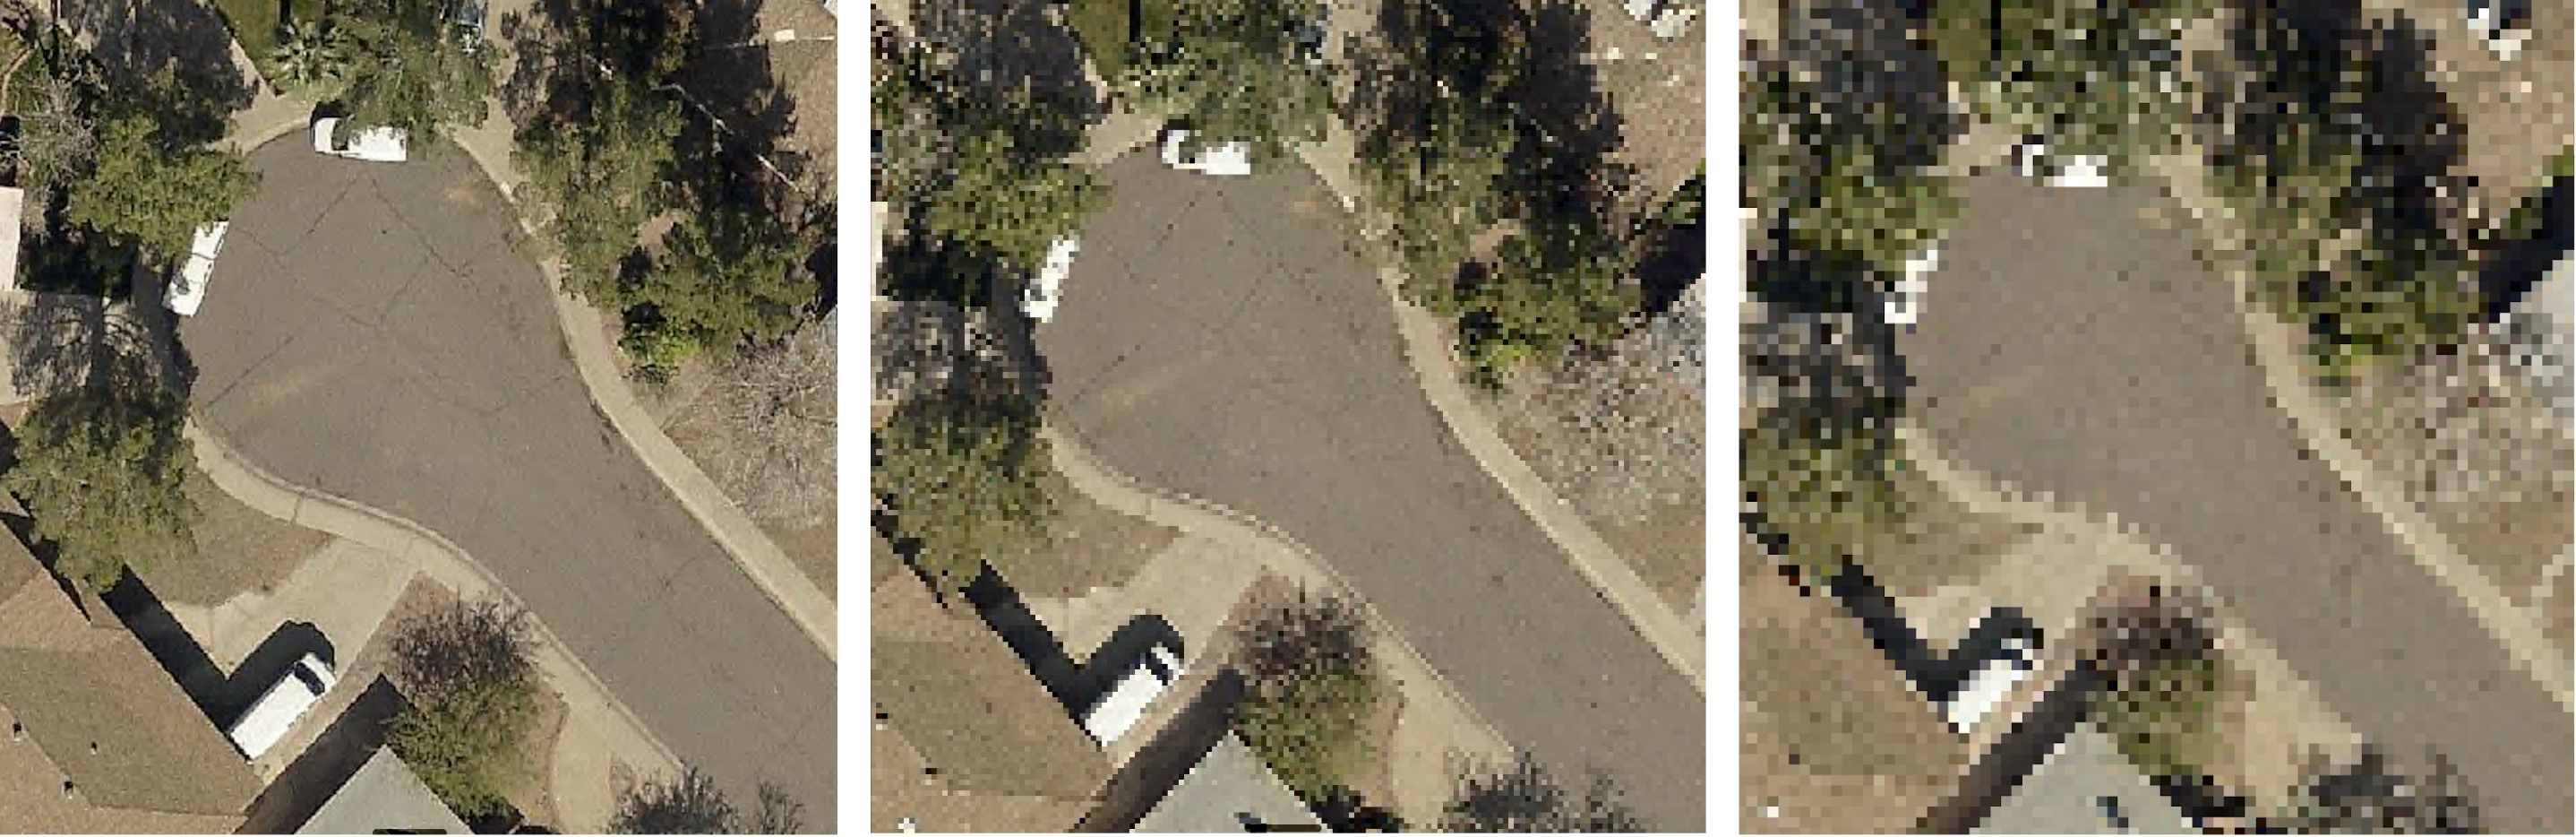
\includegraphics[width=\textwidth]{Figures/arz_7_res_compare.png}
\caption[Resolution Comparison]{
Comparison between different resolutions. 
From left to right, where
(a) has 10cm between samples, 
(b) has 0.5 meter spacing and 
(c) has 1.0 meter spacing. 
With the decrease in resolution,
it becomes harder to capture the boundary detail of the edges  of sidewalks.}
\label{fig:vhr_compare}
\end{figure}
% \todo{change dpi to 5 meter scale. make it worse.}

\ac{GSD} is the distance on the ground between the centers of pixels in an aerial image; it is
inversely related to the resolution of the image. \ac{VHR} imagery captures photographic details
with a vary small \ac{GSD} -- often less than one meter. Much of the data we target is at
resolutions well below one meter between samples; for example \ref{fig:vhr_compare}(a) has \ac{GSD}
of 10cm. The ability to resolve details at a small \ac{GSD} is advantageous for building
extraction, road detection or image segmentation~\cite{FREIRE20141, 10.1007/BFb0015525,
10.1007/978-3-642-15567-3_16}, although with additional detail one often encounters noise
or clutter that may interfere with object segmentation. \ac{VHR} aerial
images contain more information and detail due to the higher resolution, which gives us the ability
to develop more complex analysis on the imagery. \figref{fig:vhr_compare}
demonstrates the difference between different resolutions within the same area. From (a) to (c), the
resolution changes from $\frac{1}{10}$ meter \ac{GSD} to 1.0 meter \ac{GSD}. With higher resolution,
it is easier to find the precise boundaries of an object or even identify thin objects at all. For
building extraction, higher resolution provides more information when dealing with complex roofs
~\cite{10.1007/BFb0015525}. For thin ribbon-features segmentation such
as sidewalks in our approach, the output may be effected by tiny discrepancies between digitized
pathways~\cite{10.1007/978-3-642-15567-3_16}. Aerial images used to make digital maps have often
been subjected to  a process called \textit{ortho rectification}, in which a digital elevation model
has been used to predict the parallax offset between pixels in the image and their position on a
map. Perspective causes objects at higher elevation to appear to shift away from the center of an
image. Ortho-rectification predicts the distortion and corrects it to make the image appear as if it
was taken by an orthographic camera. However, most elevation models are very coarse compared to the
thin features that can be seen in \ac{VHR} images, and small errors in the ortho-rectification
process may cause thin or small features to appear to shift. It is also common for images to be
subjected to resolution ``enhancing'' operations such as pan-sharpening that attempt to artificially
increase the apparent resolution of the image. Prior image processing and rectification operations are 
useful but they can also challenge attempts to segment objects based only on object material or texture. 
 
\section{\ac{OSM}}\label{sec:osm}
\begin{figure}[H]
    \centering
    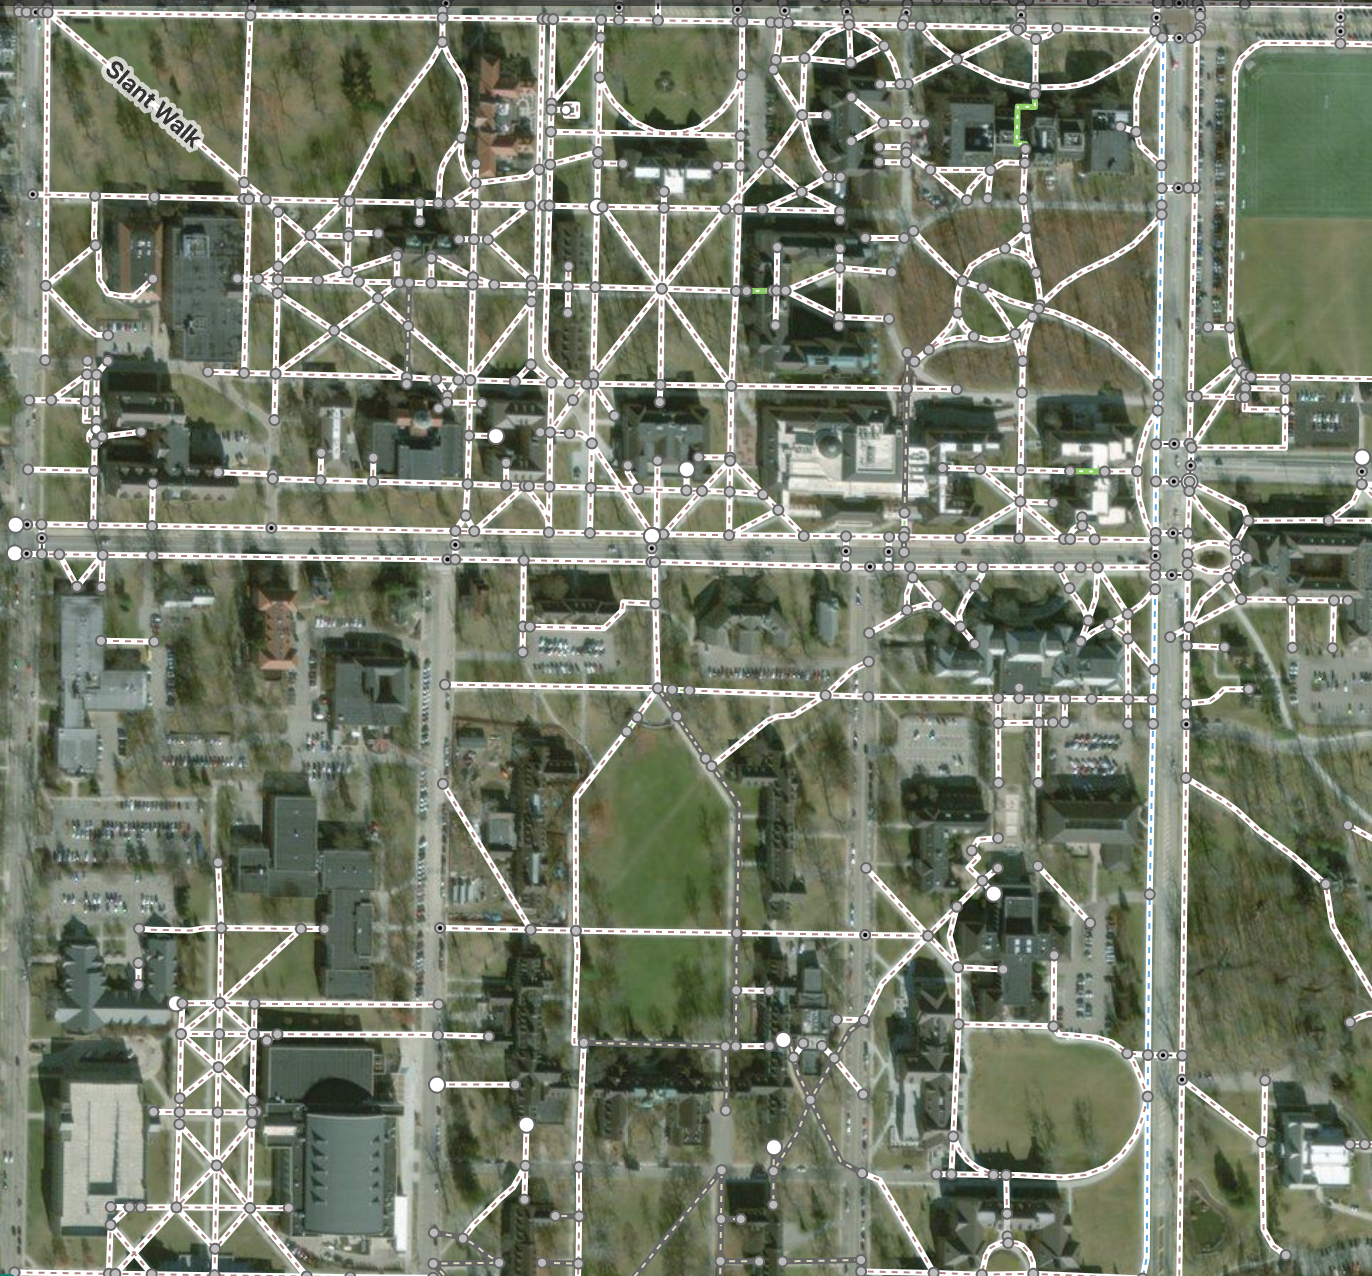
\includegraphics[width=0.85\textwidth]{Figures/oxford_path_data_osm.png}
    \caption[\ac{OSM} Walking Path]{A demonstration of actual walking path data from \ac{OSM} \cite{OpenStreetMap}. 
    The figure shows the campus of Miami University in Oxford, Ohio in USA. 
    Row 2 shows a zoomed version of the imagery.
    The sidewalk misses in the path data (left), the path is offset compared to the actual sidewalk(right).}

    \label{fig:osm_oxford_path}
\end{figure}

\ac{OSM} stands for Open Street Map, which was founded by Steve Coast in 2004~\cite{lasPiñas, OpenStreetMap}. 
\ac{OSM} is a collaborative project that allows users to generate a free editable map of the world~\cite{4653466}.
%Rather than the map itself, \ac{OSM} generates the data with the map information that across most of the world as primary output. 
It also allows users to develop the map data with portable 
satellite navigation devices, for example by recording GPS trails. 
With all these convenient features, \ac{OSM} is a helpful tool for  map analysis
 and feature segmentation~\cite{10.1007/11744078_9}. 
\figref{fig:osm_oxford_path} shows that \ac{OSM} supports features such as footpaths, roads, buildings, 
and others. There are public APIs that provide users with the ability to extract the \ac{GIS} data for 
any individual feature. 
Although crowd-sourced map data is a powerful resource, it may also lead to the issue of
missing, inaccurate or invalid data when we rely on the data set for sidewalk localization. 
In addition any GIS data may no longer match imagery as structures change over time.

\section{\ac{CRF}} \label{sec:crf}
\acfp{CRF} are is a class of statistical graphical modeling methods that often applied in pattern recognition and machine learning~\cite{MAL-013}. 
As a type of discriminative undirected probabilistic graphical model, \acp{CRF} are commonly used for segmenting, labeling or parsing of sequential data, such as in computer vision, structure segmentation and object recognition~\cite{RuizSarmiento2015UPGMppA, 1315232, lafferty2001conditional}. 
For road segmentation, several approaches are able to locate the precise 
boundaries by treating it as a \ac{CRF} problem~\cite{ActiveContou09, Achanta:149300}. 


\section{\ac{GMM}}\label{sec:gmm}

\acfp{GMM} represent probability densities as a mixture of (e.g. multivariate) normal distributions 
~\cite{sridharan2014gaussian}. A \ac{GMM} is a probabilistic model for representing normally
distributed subpopulations within an overall population. A \ac{GMM} can often  be estimated using
the \ac{EM-GMM} algorithm based on data points which are sampled from a mixture of Gaussian distributions. It can
be used in common computer vision tasks such as background and foreground
subtraction~\cite{1333992}. For road segmentation, we can treat the problem as separating foreground
(colors within a ribbon) from the complex background (non-ribbon colors). \figref{fig:gmm_sample_1}
demonstrates the comparison between foreground and background \acp{GMM} on a sample walking path,
with the density estimate for each pixel shown in gray-scale. For foreground density estimation,
which we show in row 1 and row 3, we treat sidewalk colors as foreground and apply the \ac{EM-GMM}
algorithm to estimate the probability density $\Pr(\Color{}|R)$ where $\Color{}$ is the event that a
color is observed in the image and $R$ is the event that we are part of a sidewalk (ribbon).
Background likelihoods are shown in row 2 and row 4, we did the opposite and estimated
$\Pr(\Color{}|\neg R)$. More details including the number of Gaussian distributions in each mixture
we use are described in section \S\ref{sec:density-estimation}, and the result of using Bayes theorem to estimate the posterior probability 
$\Pr(R|\lambda)$ that a pixel is part of a ribbon are shown in \figurename{}\ref{fig:GMM_Sample_2}

\begin{figure}[H]
\centering
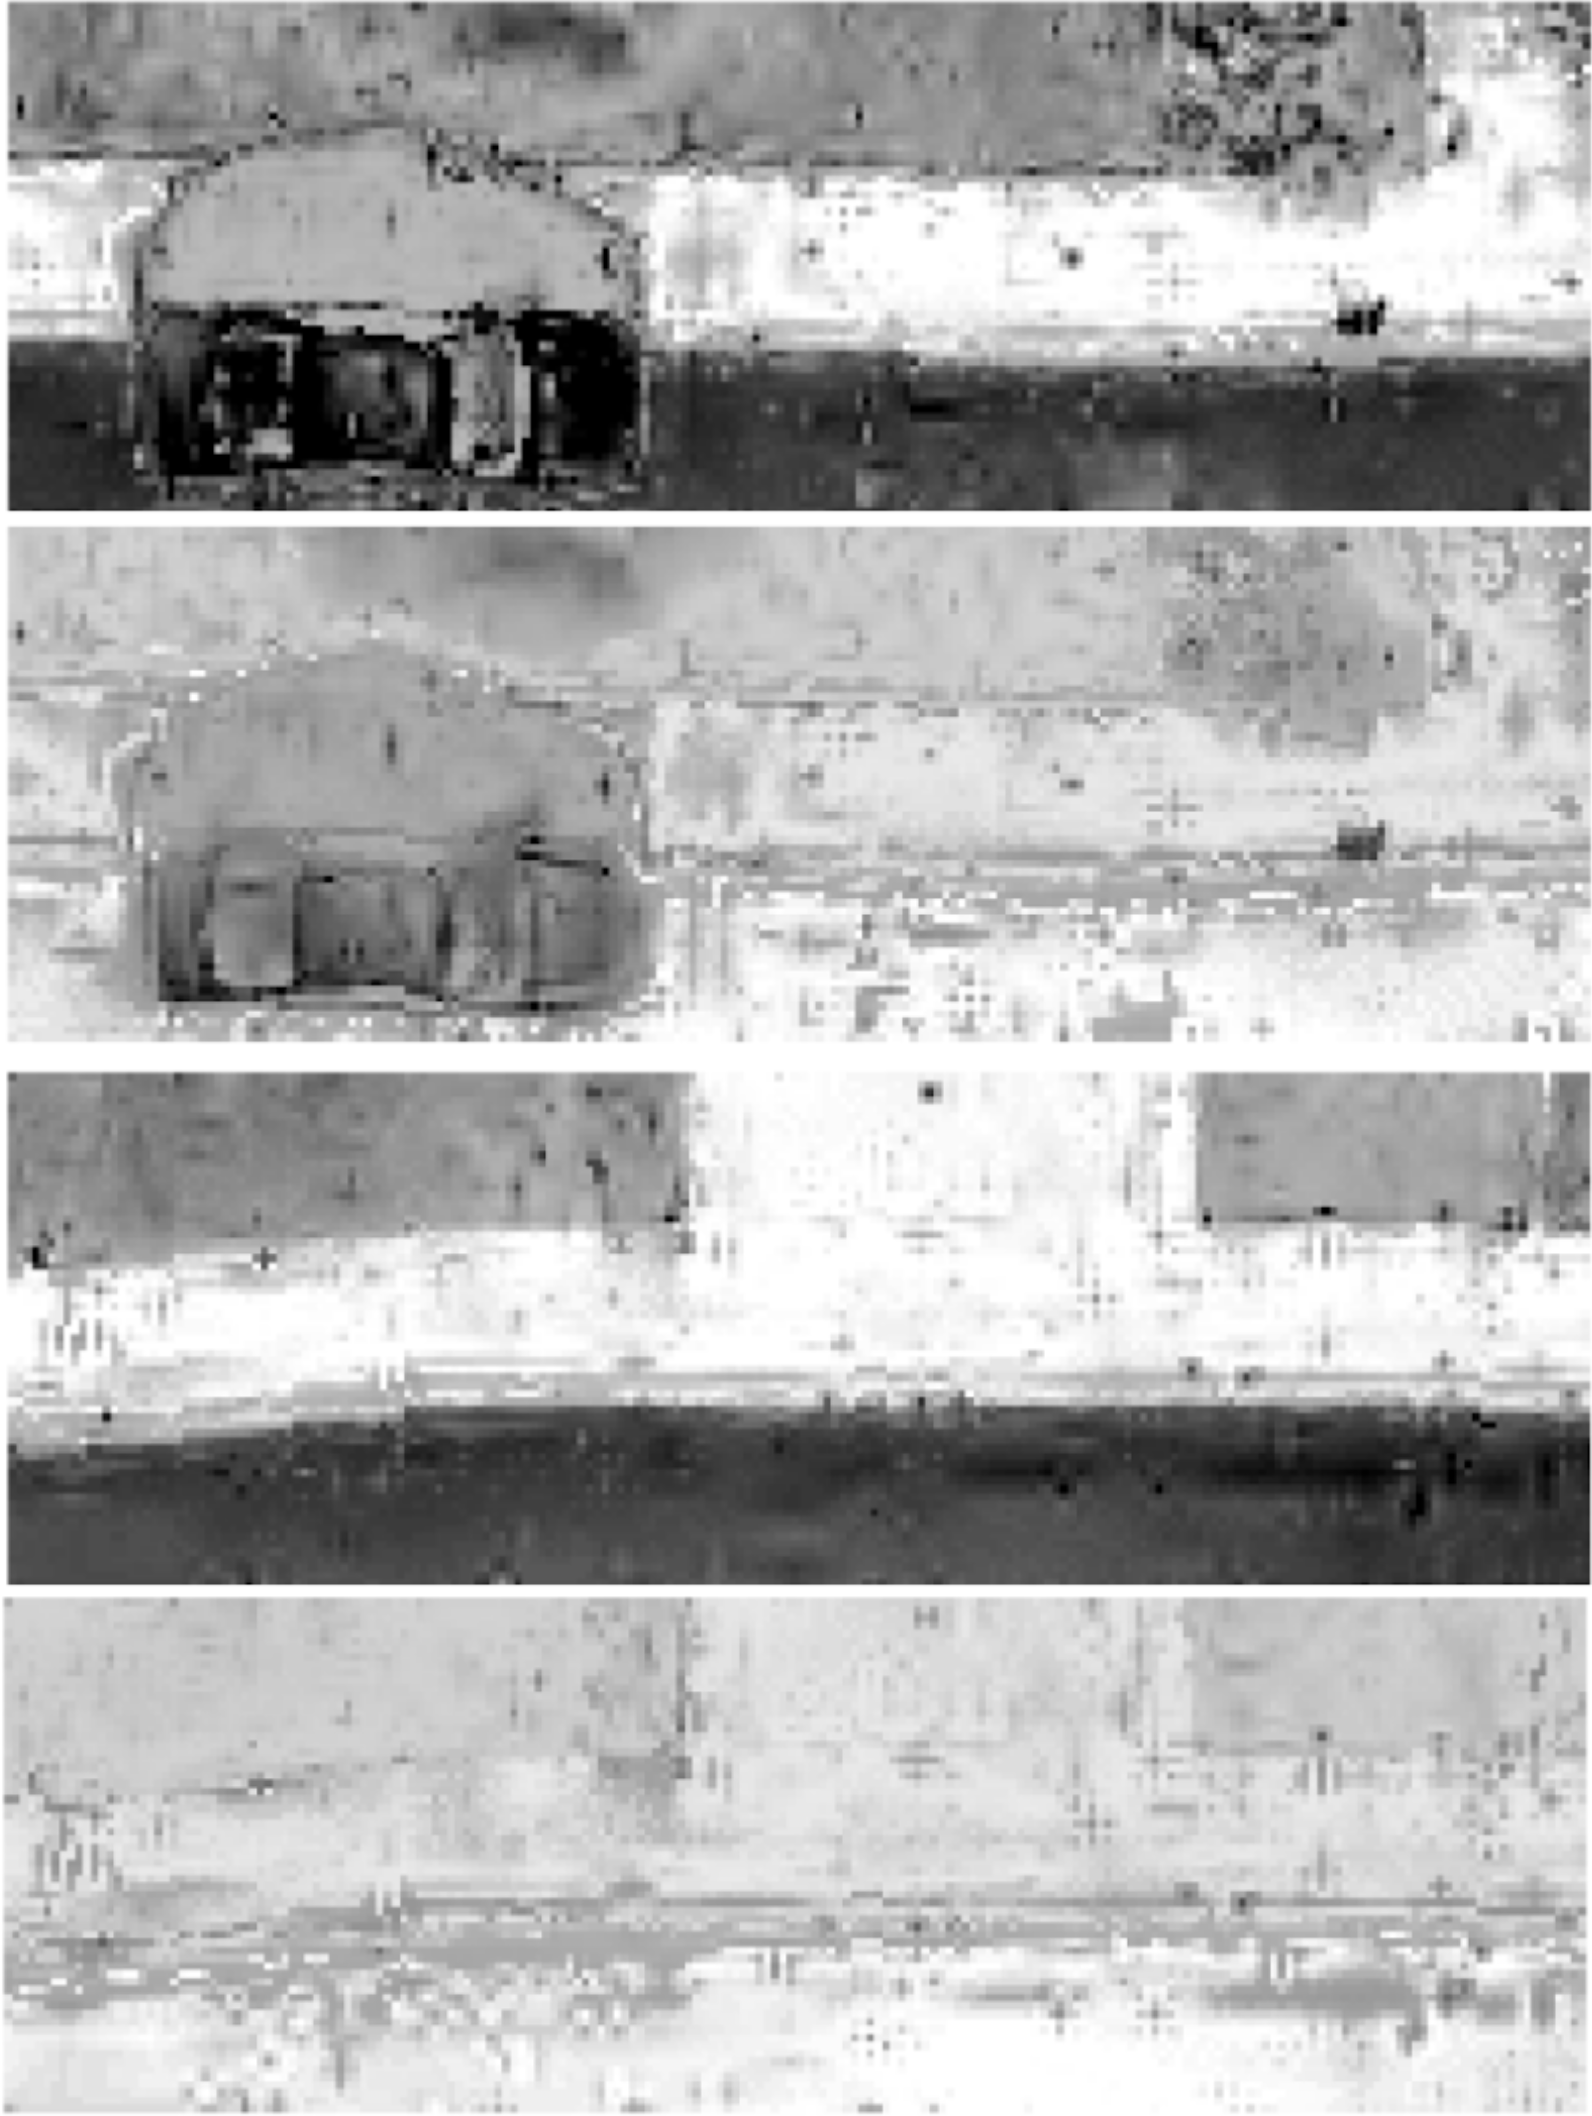
\includegraphics[width=0.85\textwidth]{Figures/GMM_needed.png}
\caption[Density Background Subtraction]{
A demonstration of the \ac{EM-GMM} algorithm on sample inputs, probability densities are shown in gray scale. 
From top to bottom, row 1 shows foreground density on a sample path, row 2 show background density on 
the same sample path as row 1. 
Row 3 and 4 show the same with a different sample path. 
A lighter color represents higher probability density.}
\label{fig:gmm_sample_1}
\end{figure}

\section{\ac{DP}}\label{sec:dp}

\acf{DP} is both a mathematical optimization method and a computer programming method \cite{bertsekas2005dynamic}. 
In 1950s \ac{DP} was invented by Richard Bellman\cite{bellman2013dynamic}. 
The main concept of \ac{DP} is to simplify a complicated problem by breaking it down into smaller overlapping sub-problems
 in a recursive manner \cite{howard1966dynamic}. 
In computer science, if a problem can divided into several overlapping sub-problems, 
each sub-problem can be recursively solved by finding its optimal solution, and if some subproblems are repeated, then 
we know that \ac{DP} is applicable. \ac{DP} is characterized by caching or \textit{memoizing}
 the solutions to repeated subproblems in a table, and the using the stored values rather than solving
 the same problem multiple times.  

Dynamic Programming has a variety of applications since it can significantly reduce the 
running-time of some algorithms \cite{bertsekas1995neuro}. 
We use Fibonacci Sequence 
$$F(n) = \begin{cases}
1 & \text{if $n=1$ or $n=2$}\\
F(n-1)+F(n-2) & \text{if $n>2$}
\end{cases}$$
to demonstrate the \ac{DP} process\cite{horadam1961generalized}. 
Figure \ref{fig:fbs}, row 1 shows that to calculate the $n^{th}$ Fibonacci number, one must 
evaluate exponentially growing number of subproblems to finish the process.
The time complexity can be reduced since we are re-calculating certain Fibonacci numbers repeatedly. 
By applying a \ac{DP} approach, we can save the previous calculated Fibonacci number and reuse it when needed.
Figure \ref{fig:fbs}, row 2, shows the same process after applying dynamic programming. Unnecessary steps are marked with a red `X'. 
By trading a linear amount of space (for caching results) to save previous calculation, we can reduce the running time from exponential to linear.

\begin{figure}[H]
\centering
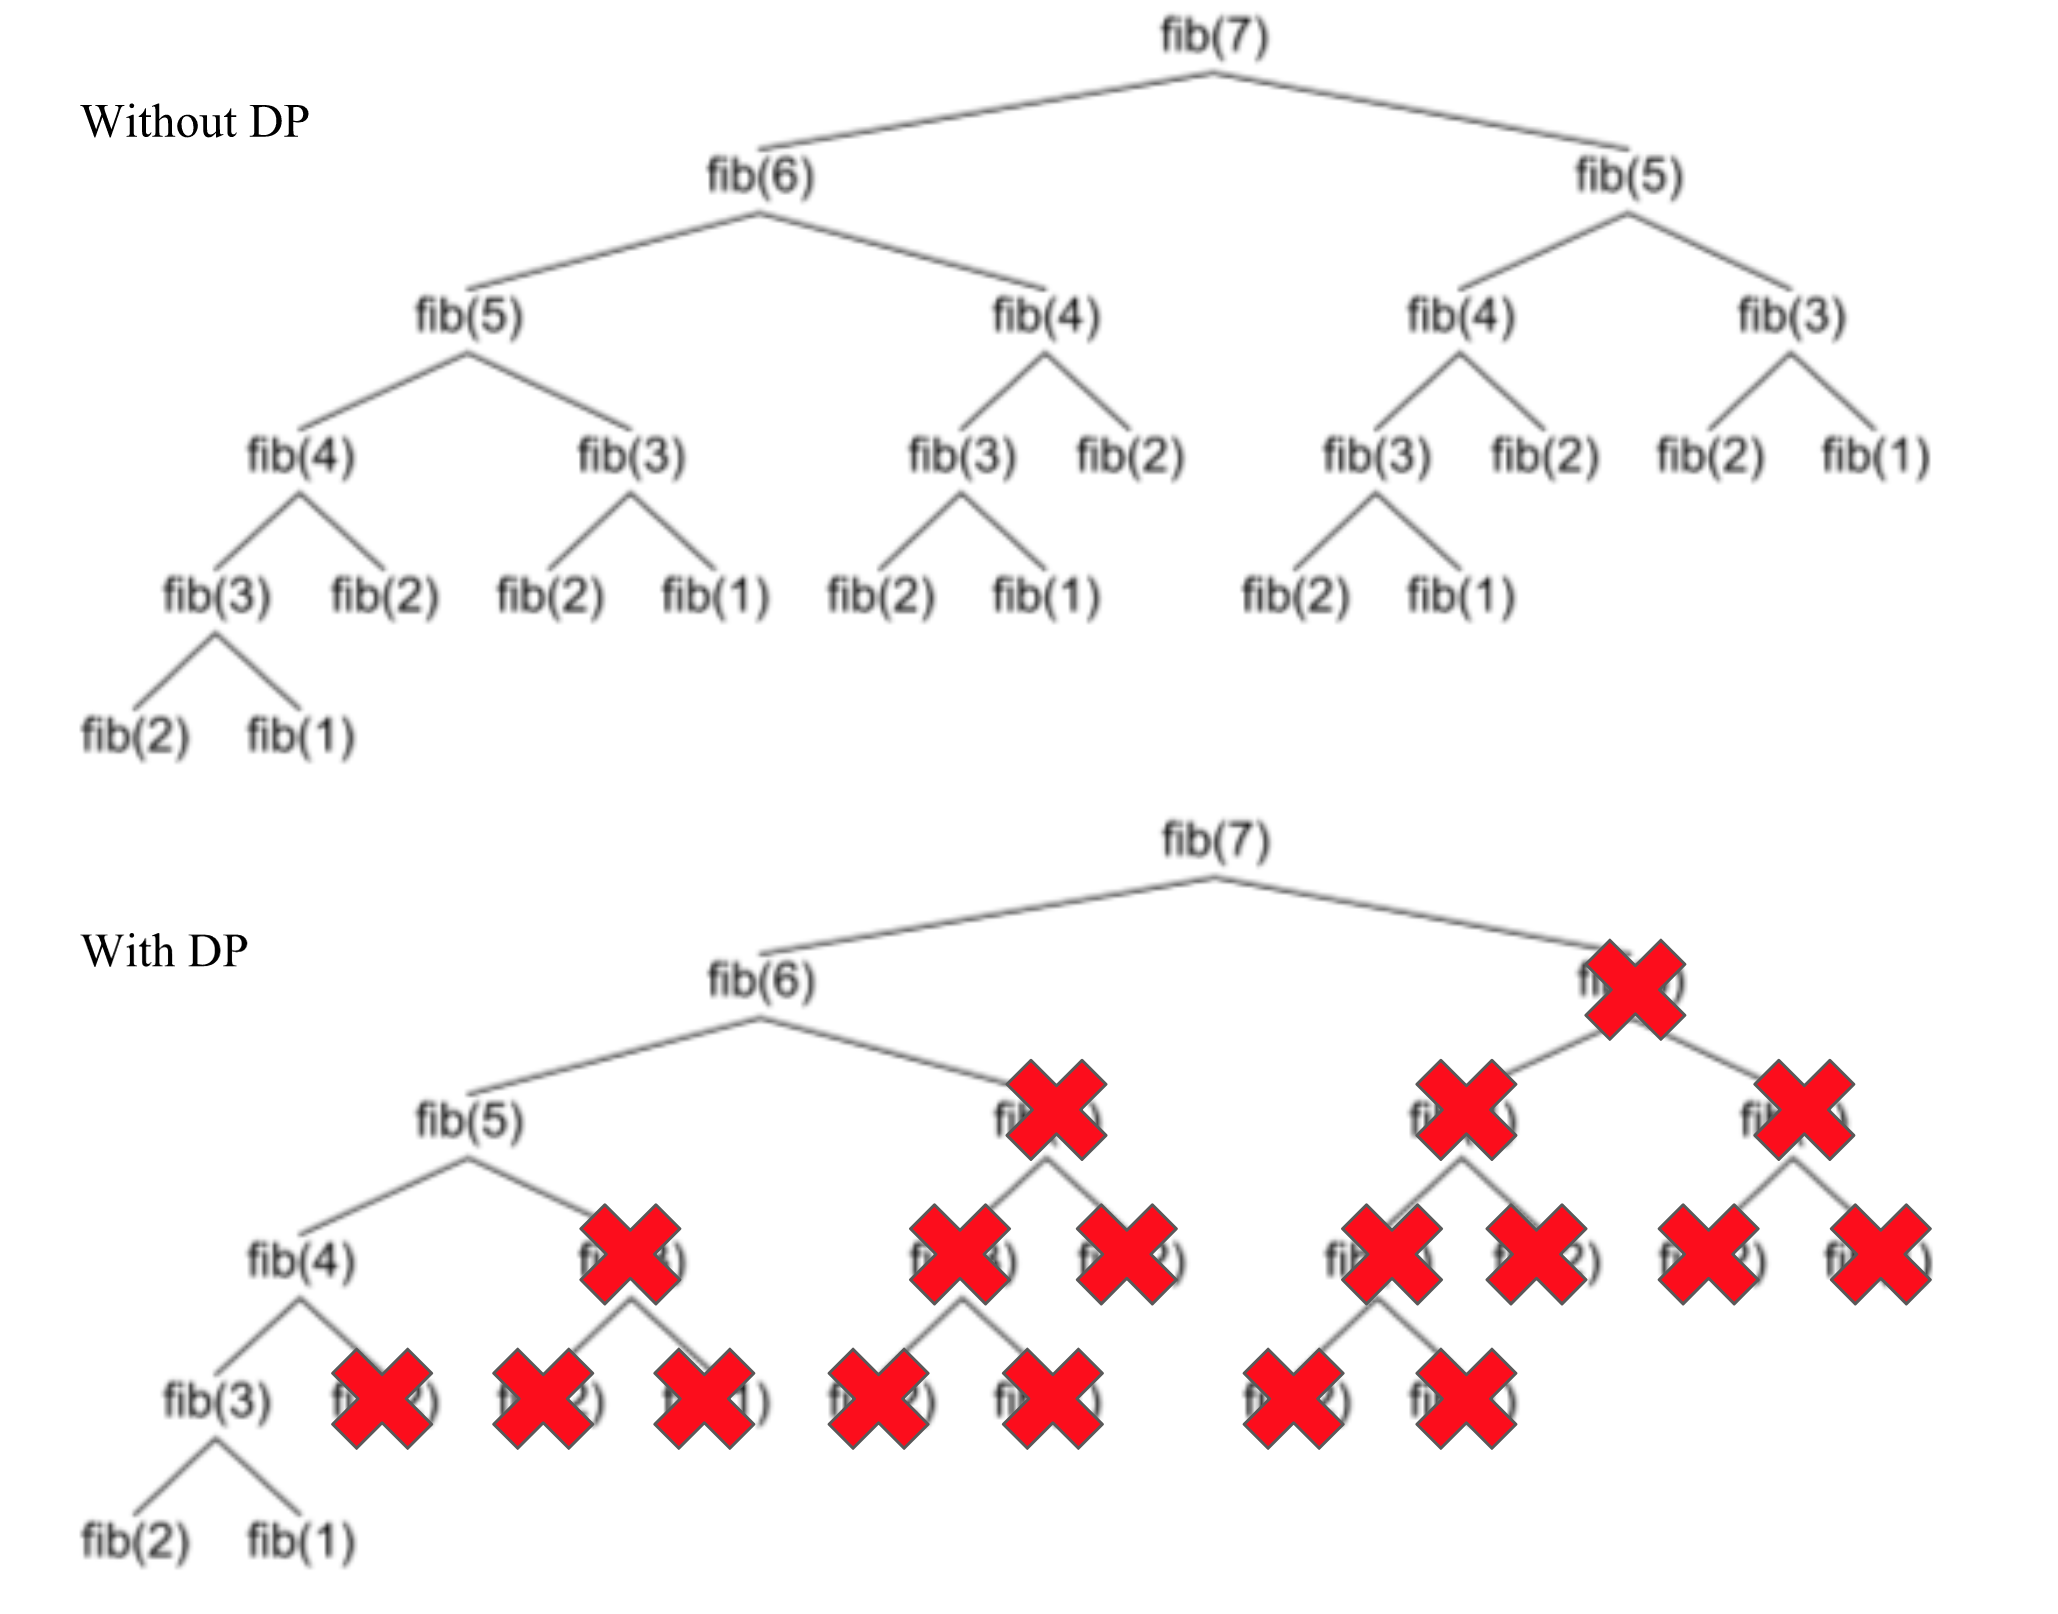
\includegraphics[width=\textwidth]{Figures/treewithdp.png}
\caption[Demonstration on Fibonacci Sequence]{
In image from \cite{stack_overflow} representing the calculation of the $7^{th}$ Fibonacci number with a recursion tree. 
Row 1 shows without applying dynamic programming, one must solve an exponential number of subproblems to calculate $n^{th}$ Fibonacci number. 
With the increase of $n$, the number of calculations increase significantly.
Row 2 shows that with dynamic programming, after saving previous calculations, 
one requires a linear number of steps (left edge of the tree) 
to calculate $n^{th}$ Fibonacci number.
We marked unnecessary steps in red ``X'' to show it can be skipped. }

\label{fig:fbs}
\end{figure}


\ac{DP} often involves first filling in a table with the \textit{optimal value} of sub-problems, and
in order to recover the sequence of decisions that led to the optimal value a process of \textit{backtracking} is used. 
\figref{fig:lcs_dp} gives a example of a famous dynamic programming problem, finding the length of the Longest Common Sequence. 
Given two strings $t_1=\langle t_{1,1}, t_{1,2}, \dots, t_{1,m}\rangle$
and $t_2=\langle t_{2,1}, t_{2,2}, \dots, t_{2,n}\rangle$, we aim to identify 
the \textit{length} of the longest subsequence that is common to both $t_1$ and $t_2$.
In this case a subproblems are prefixes of the strings $t_1$ and $t_2$.
Once we know the lengths of the longest subsequences for every subproblem, we can use 
backtracking to generate the longest subsequence itself. 
The longest common sequence is useful for geospatial processing, for example it has been use for intersection detection from GPS
traces~\cite{Xie2017DetectingRI}.

The length of the $\mathtt{LCS}$ for prefixes of length $i$ and $j$ is determined recursively as
$$
\mathtt{LCS}(i, j) = \begin{cases}
\mathtt{LCS}(i - 1, j - 1) + 1 & \text{if $t_{1, i} = t_{2,j}$}\\
\max\left[
\mathtt{LCS}(i-1, j),
\mathtt{LCS}(i, j-1)
\right] 
& \text{else}\\
\end{cases}
$$
and a subproblem is solved for each pair of sizes $i,j$ in the table of \figref{fig:lcs_dp}.
As each subproblem is solved, one of three choices was made in the recurrence (depicted by arrows in the table). 

By following the arrows in \textit{reverse} starting at $m,n$, one is able to determine which
 symbols were common to both strings in the longest subsequence. 


\begin{figure}
\centering
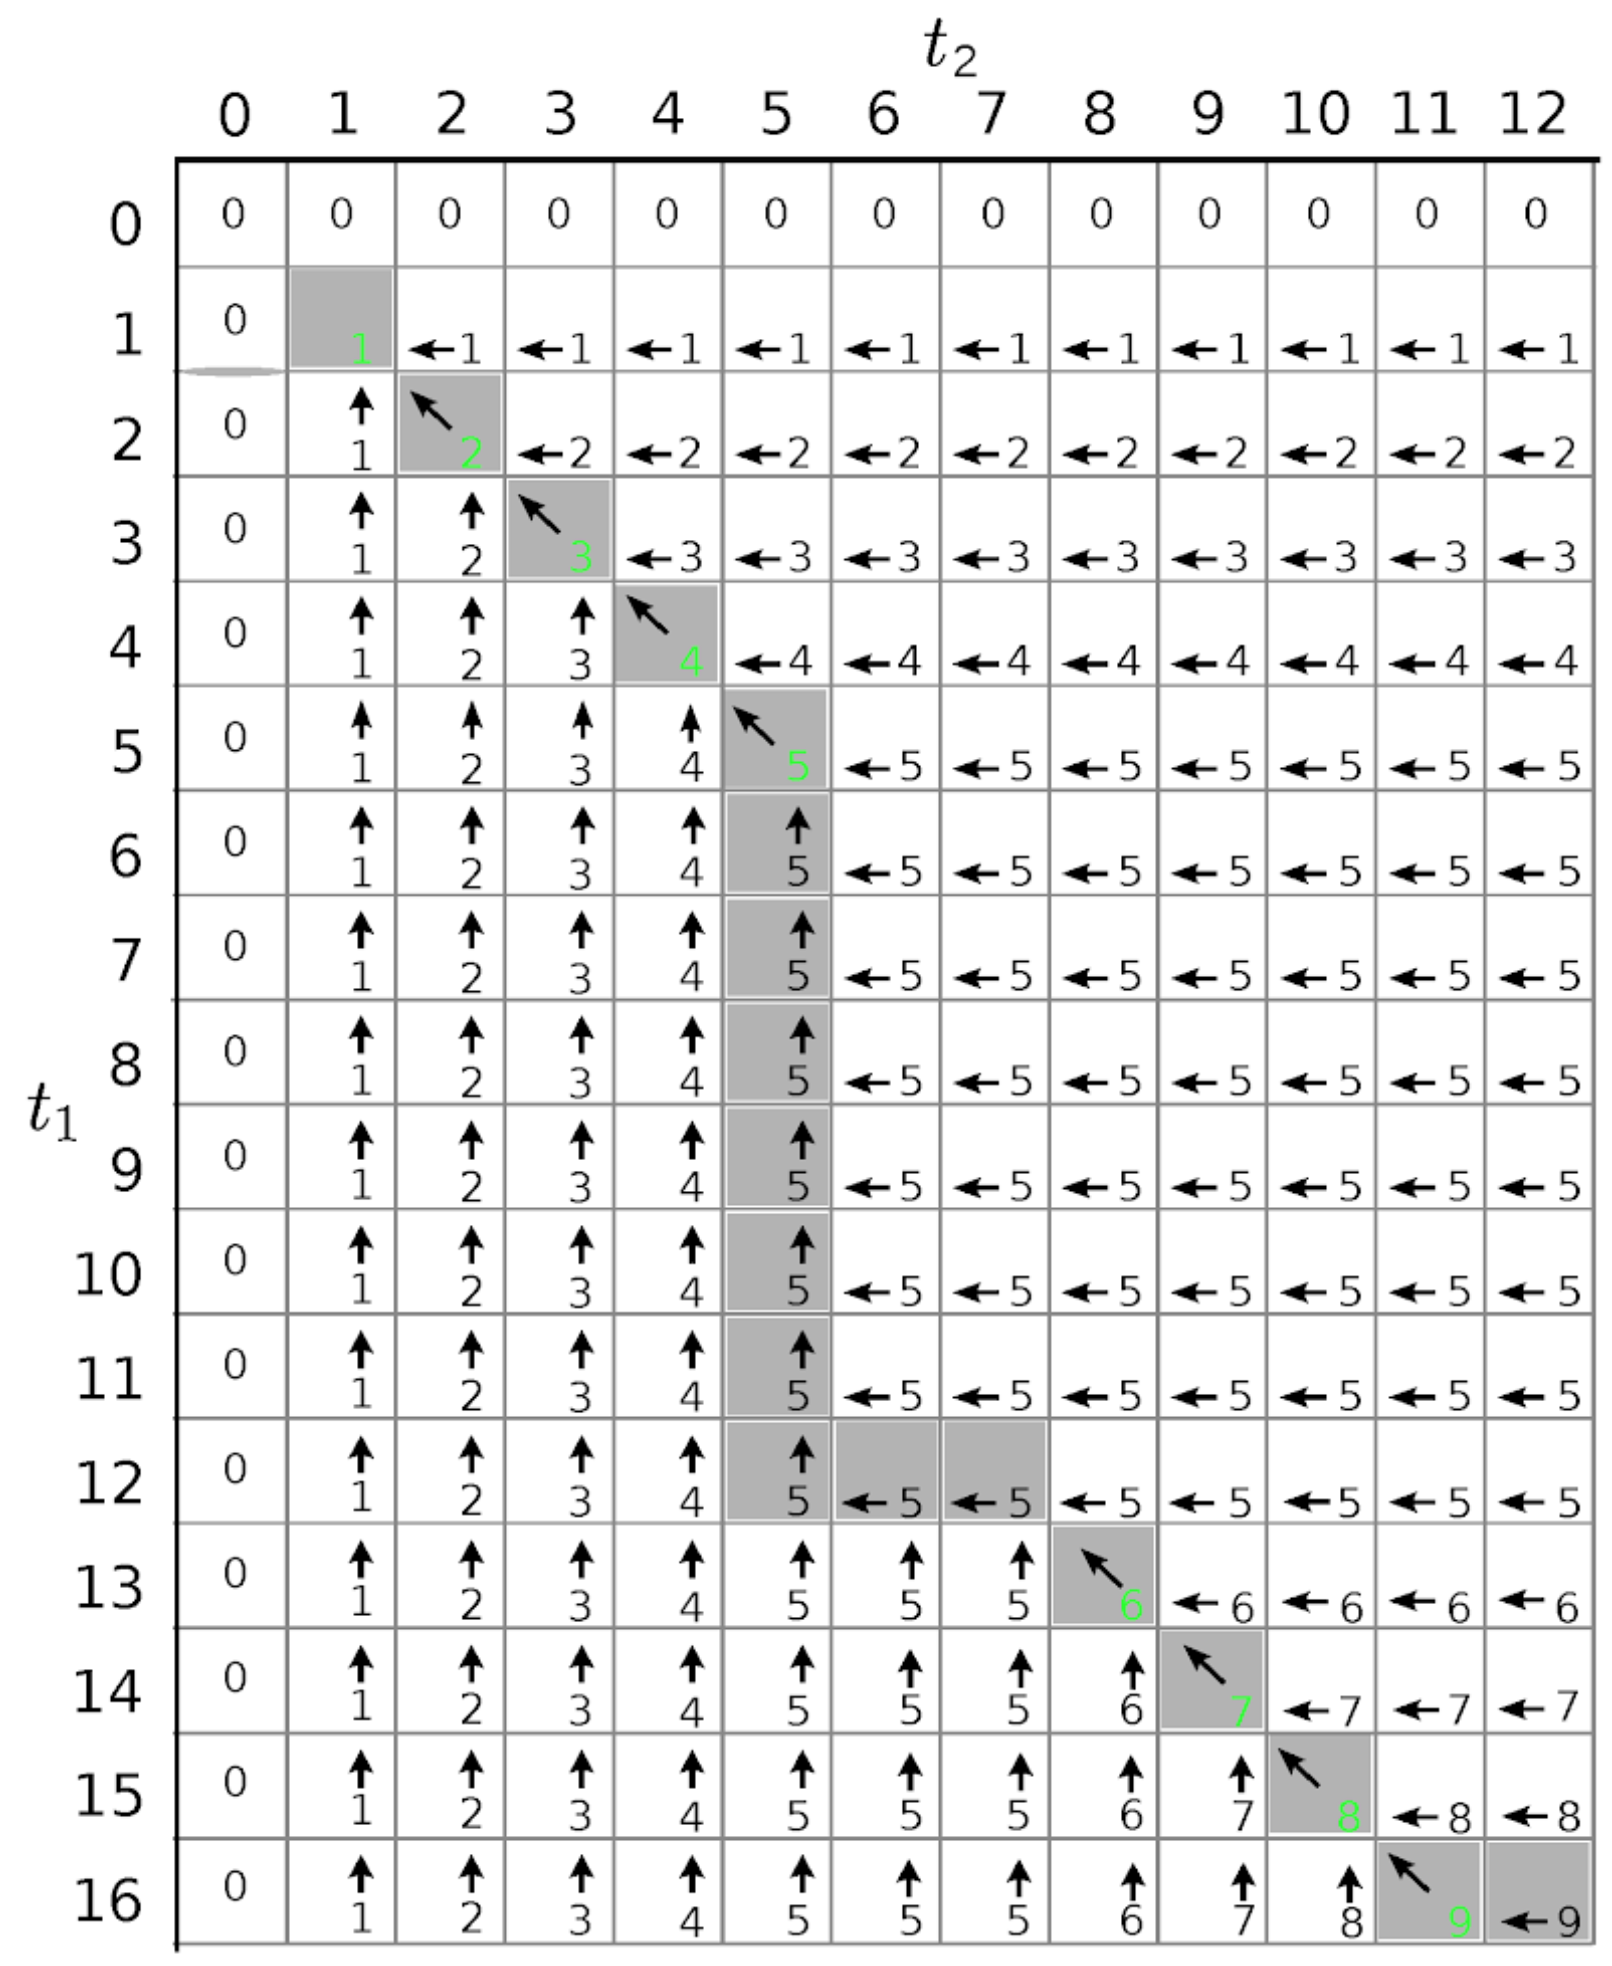
\includegraphics[width=0.9\textwidth]{Figures/longest_common_sequence.png}
\caption[Demonstration on Longest Common Sequence]{
Dynamic Programming demonstration with longest common sequence from \cite{Xie2017DetectingRI}. 
Similar to our approach, to find the longest common sequence, one first fills the table using \ac{DP} and
 then backtracks to find the optimal path. 
}
\label{fig:lcs_dp}
\end{figure}


% \begin{figure}
%     \centering
%     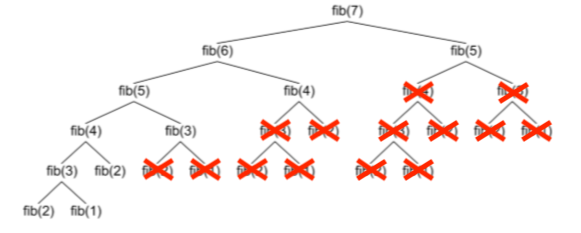
\includegraphics[width=\textwidth]{Figures/QVSdv_DP.png}
%     \caption[Demonstration on Fibonacci Sequence with \ac{DP}]{Representing the calculation of Fibonacci Sequence ($7^{th}$) with binary tree. With dynamic programming, after saving previous calculation, it's only require linear time steps to calculate $n^{th}$ Fibonacci number. We marked unnecessary steps in red X to show it's can be skipped.
%     }
%     % \cite{stack_overflow}
%     \label{fig:fbs_dp}
% \end{figure}

% \section{Street Network Extraction}
% boss paper, 2018 cvpr, they don't gurant to find the center of road.

